\chapter{Aplicación Web}
\label{cap:aplicacion}

Parte del trabajo realizado en esta tesis consiste en el desarrollo de una aplicación Web para presentar la información en tiempo real. 
%
El objetivo principal del desarrollo de esta aplicación no es el diseño del software ni de las interfaces, si no más bien, poner en producción una prueba de concepto que permite validar su utilidad como herramienta de apoyo para los sismólogos del Centro Sismológico Nacional.


La aplicación debía permitir a los usuarios identificar las características de los eventos rápidamente, es decir, identificar la hora y el lugar donde ocurre el sismo y el impacto que tuvo en la red social.
%
Además, para los usuarios e investigadores es muy valioso tener la posibilidad de explorar datos históricos. Para cumplir con este objetivo la aplicación permite pausar el refresco de información y cargar datos recopilados para fechas anteriores.  
%
La aplicación está disponible en \url{http://www.twicalli.cl}.

%A continuación se explican las visualizaciones utilizadas para presentar la información, el diseño que integra cada una de las partes y las interacciones disponibles para que el usuario explore los datos.

\section{Visualización de datos}
\label{sec:visualizacion}

La información que se desea presentar en la aplicación Web consiste principalmente en datos geográficos y temporales. 
%
En la prueba de concepto desarrollada se proponen algunas visualizaciónes básicas para que los usuarios identifiquen rápidamente cuándo está ocurriendo un sismo, dónde se percibe y lo que las personas están comentando al respecto.
%
En esta sección se explica en qué consiste cada una de estas visualizaciones.


	\subsection{Temporales}
	
	\begin{figure}[ht]
	  \centering
	  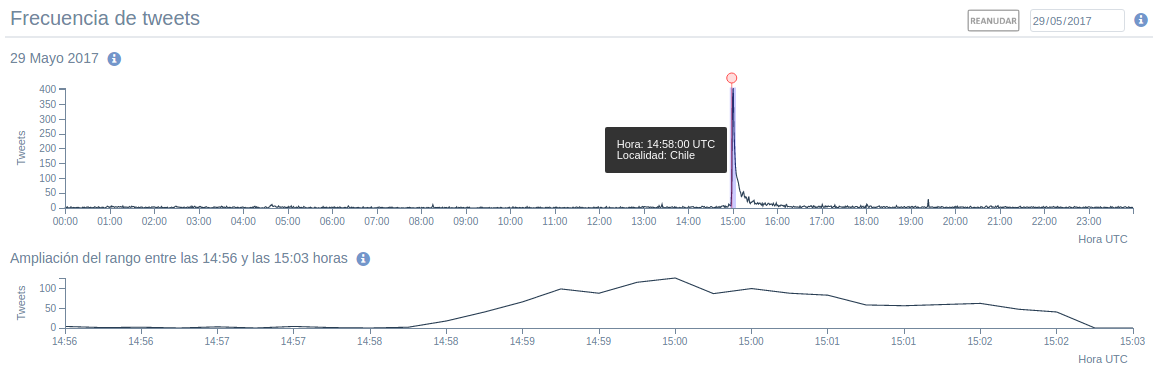
\includegraphics[trim={0 0 0 0}, clip, width=\textwidth]{imagenes/linea_de_tiempo_interactive.png}
	  \caption{Visualización de la frecuencia de \textit{tweets} de un día completo en intervalos de 60 segundos y de la frecuencia de \textit{tweets} de la zona seleccionada en intervalos de 15 segundos.}
	\label{fig:timeline}
	\end{figure}
		
	
	Para visualizar los datos temporales, se utiliza una señal interactiva similar a un gráfico de línea, que se actualiza a medida que pasa el tiempo y que muestra la cantidad de \textit{tweets} publicados en cada momento.
	%
	La imagen \ref{fig:timeline} corresponde a la visualización de los datos recolectados el día 29 de Mayo del 2017.
	%
	La primera señal muestra los datos recolectados en un rango de un día y la segunda señal muestra el rango seleccionado amplificado. Por defecto, están seleccionados los últimos 30 minutos.
		
	Mediante esta visualización es posible identificar rápidamente cambios en el comportamiento típico de los usuarios.
	%
	Además el sistema marca automáticamente los puntos de interés, en este caso, los puntos en donde inicia un sismo. 
	%
	Los usuarios pueden interactuar con esta visualización, ya sea seleccionando un rango de tiempo o haciendo \textit{click} en un punto de interés, lo que permite obtener información más detallada de el periodo de tiempo seleccionado. 
	
	
	\subsection{Geográficos}
	
	\begin{figure}[ht]
	\centering
	\subfloat[Mapa del mundo con \textit{tweets} geolocalizados.]{
		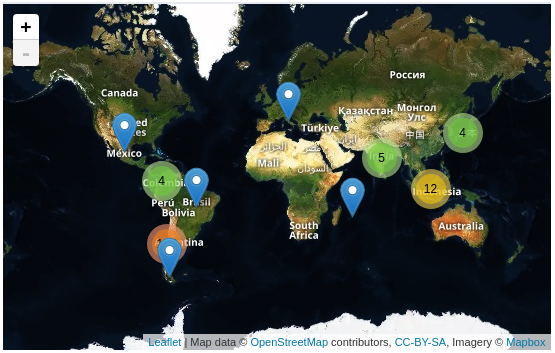
\includegraphics[height=140pt]{imagenes/worldmap.png}
		\label{fig:worldmap-out}
	}
	\hfill
	\subfloat[Mapa ampliado a la zona afectada por el sismo.]{
  		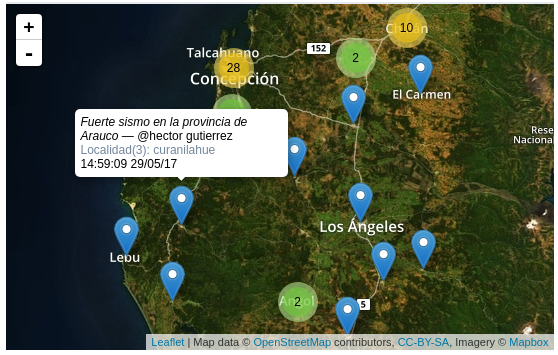
\includegraphics[height=140pt]{imagenes/worldmap-maxzoom.png}
  		\label{fig:worldmap-zoom}
  	}
  	\caption{Mapa interactivo con marcadores para cada tweet geolocalizado y agrupados en base a la distancia que existe entre ellos. Las imagenes corresponden a un sismo ocurrido cerca de  Concepción, Chile, el 29 de Mayo del 2017.}
  	\label{fig:worldmap}
  	\end{figure}
	 	
	  	
	Como se mencionó en el capítulo \ref{cap:geocodificacion} se intenta obtener la mayor cantidad posible de información geográfica. 
	%
	Esto es muy útil ya que, a pesar de no ser 100\% confiable, entrega una buena aproximación de la percepción de un sismo. 
	%
	Saber donde se encuentran los usuarios que reportan un sismo nos permite identificar las áreas afectadas y el alcance geográfico de cada evento. 
	%

	
	Para mostrar esta información se utilizan dos tipos de mapas, el primero consiste en un mapa de calor. 
	%
	La figura \ref{fig:heatmap} visualiza los datos recolectados durante los 15 minutos posteriores a un evento sísmico ocurrido el 29 de Mayo cerca de Concepción. 
	%
	En ella se puede observar la zona en donde se publicaron un mayor número de \textit{tweets} y cómo esto se modifica en el tiempo.
	%
	%Como se puede observar, la imagen muestra una mancha roja un poco más abajo de Santiago. 
	%
	%Esto se debe a que este mapa no se encuentra normalizado. 
	%
	%Sin embargo el usuario tiene la opción de escoger ver el mapa normalizado por población regional, lo que permite observar más claramente que el evento ocurrió más al sur de Chile. 
	%
	%El mapa que muestra los mismos datos pero normalizados por región se muestra en la figura \ref{fig:heatmap-normalizado}.
	
	
	El segundo tipo de mapa consiste en un visualización interactiva del mapa del mundo con marcadores para cada tweet relacionado con alguna localización.
	%
	Para una mejor visualización, los datos se agrupan en base a su cercanía y se van separando en grupos más pequeños a medida que el usuario amplía el mapa o hace \textit{click} en cada grupo. 
	%
	La figura \ref{fig:worldmap-out} muestra la visualización durante un sismo en Chile y la figura \ref{fig:worldmap-zoom} muestra el mismo instante pero con el mapa ampliado a la zona con mayor número de marcadores.
	%
	La visualización permite identificar rápidamente los lugares afectados, en este caso, en el mapa \ref{fig:worldmap-out} se identifica un grupo grande en Chile y a medida que se amplía esa zona, en el mapa \ref{fig:worldmap-zoom} se identifica un grupo numeroso en Concepción (ciudad muy cercana al epicentro) y las ciudades aledañas.
	
	\begin{figure}[!ht]
	  \centering
	  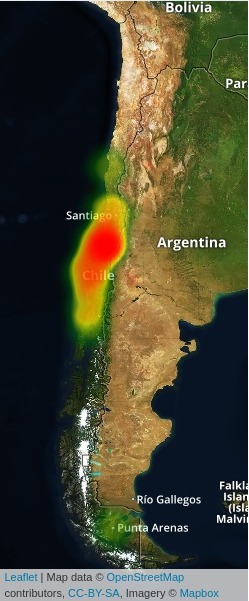
\includegraphics[trim={0 0 0 0}, clip, width=0.4\textwidth]{imagenes/heatmap.png}
	  \caption{Mapa de calor construido a partir de las coordenadas geográficas inferidas de los \textit{tweets} publicados durante un sismo en Concepción}
	\label{fig:heatmap}
	\end{figure}
  	

\section{Usuarios de la Aplicación}

Los usuarios finales de la aplicación son:

\begin{enumerate}
\item Sismólogos de las oficinas del Centro Sismológico Nacional de la Universidad de Chile (CSN)
\item Personas no expertas en sismología que deseen visitar el sitio Web
\end{enumerate}

\section{Diseño de la Aplicación}

El objetivo principal de la aplicación Web es presentar los datos a los usuarios expertos, es decir, a los sismólogos de las oficinas del CSN. 
%
La aplicación será visualizada en las pantallas de monitorización ocupando pantallas ordenadas verticalmente, además se desea poder extraer la información relevante sin la necesidad de interacción.
%
Por otro lado, la aplicación que queda disponible para el resto de los usuarios debe ser fácil de comprender. 


Es de interés poder observar los datos en tiempo real y también se desea poder explorar la información de eventos pasados. 
%
Para cada evento se presenta información de geolocalización. 


Teniendo en cuenta los puntos antes mencionados se desarrollan dos vistas de la aplicación que presentan la misma información. 
% 
Las figuras \ref{fig:webapp} y \ref{fig:webapp_csn} muestran la vista de la aplicación disponible de manera pública y la utilizada por el CSN respectivamente. 
%
En ella se observan las visualizaciones descritas en la sección \ref{sec:visualizacion} y el listado de \textit{tweets}, que permite a los usuarios comprender mejor el evento. 

	\begin{figure}[ht]
	  \centering
	  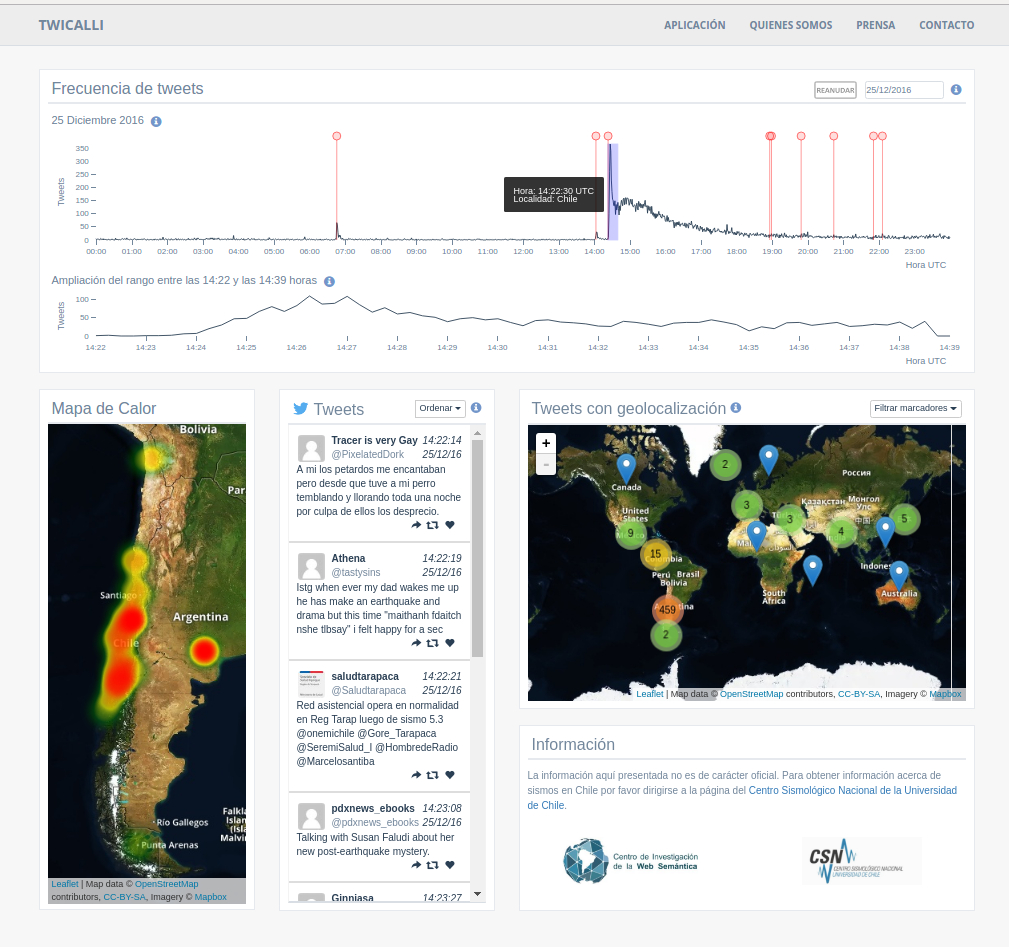
\includegraphics[trim={0 0 0 0}, clip, width=\textwidth]{imagenes/aplicacionexplorar.png}
	  \caption{Vista de la aplicación Web disponible públicamente}
	\label{fig:webapp}
	\end{figure}
	
	\begin{figure}[ht]
	  \centering
	  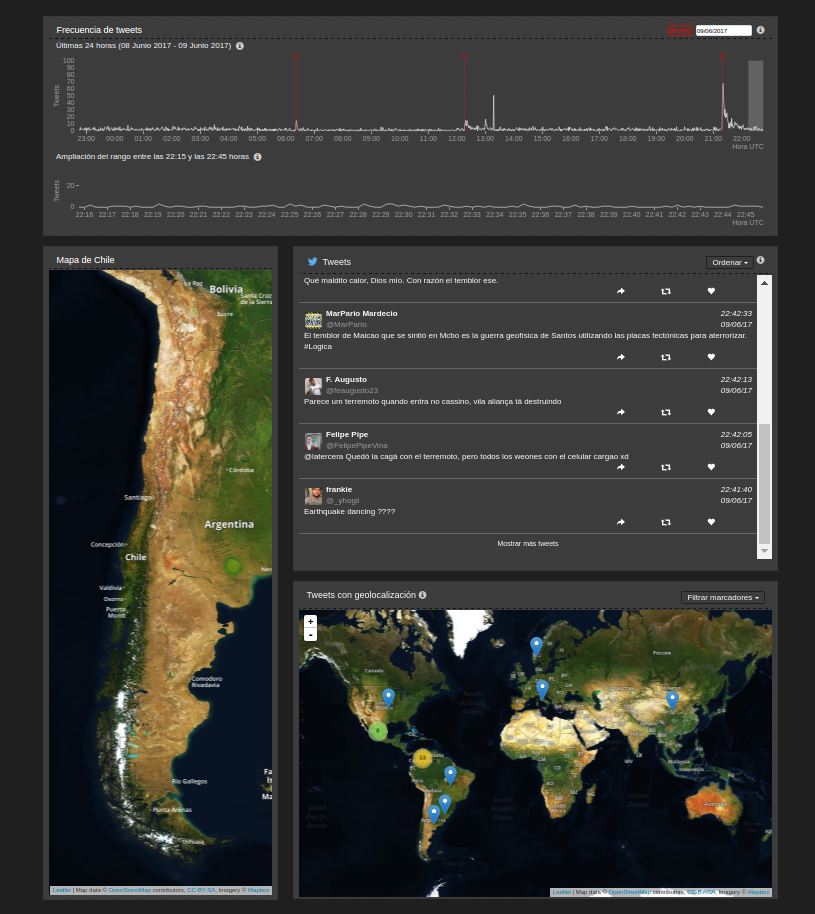
\includegraphics[trim={0 0 0 0}, clip, width=\textwidth]{imagenes/aplicacionexplorar_csn.png}
	  \caption{Vista de la aplicación Web utilizada por usuarios del CSN}
	\label{fig:webapp_csn}
	\end{figure}


Gracias a las iteraciones y la retroalimentación de los usuarios expertos se pudo identificar algunas mejoras, principalmente en la vista que visualizarán en las pantallas del CSN:

\begin{enumerate}
\item Preferencia por el uso de un mapa en el que se distinga el relieve del terreno y las fallas geográficas del borde costero chileno.
\item Selección de los colores utilizados en el mapa de calor y los marcadores para que no se confundan con los colores del mapa. 
\item Preferencia por el uso de una paleta de colores oscura para el fondo de la aplicación, debido a que el fondo blanco en las pantallas de monitorización cansa la vista.
\end{enumerate}


\section{Interacciones}

La aplicación Web por defecto presenta los datos en tiempo real correspondiente a los últimos 30 minutos.
La línea de tiempo del día completo se actualiza cada 1 minuto y la línea de tiempo amplificada se actualiza cada 15 segundos. 
Además cada 1 segundo se consulta si hay nuevos \textit{tweets} y de ser así se dibujan en los mapas y en la parte superior de lista de tweets.  

Los usuarios pueden interactuar con la aplicación y en caso de hacerlo la actualización automática se detiene, pudiendo reanudarse en cualquier momento haciendo \textit{click} en el botón \textit{reanudar} de la parte superior derecha de la línea de tiempo. 

Las interacciones disponibles son: 

\begin{itemize}
\item Seleccionar un largo de tiempo de la línea de tiempo principal. Esto permite actualizar la información en el resto de la página, mostrando el rango de tiempo amplificado y la información de los \textit{tweets} publicados durante ese rango de tiempo. 
\item Hacer \textit{click} en un marcador rojo de la línea de tiempo principal, el cual representa la ocurrencia de un evento. Esta acción selecciona automáticamente el rango en el que aumentó el número de \textit{tweets} relacionados a ese evento y actualiza la información del resto de las visualizaciones de la misma forma que la interacción anterior. 
\item Hacer \textit{click} en los marcadores del mapa que están agrupados para desagruparlos.
\item Hacer \textit{click} en los marcadores desagrupados para mostrar información específica del \textit{tweet}.
\item Seleccionar una fecha para mostrar información de un día anterior. 
\end{itemize}



